\documentclass[12pt]{article}
\oddsidemargin   0mm
\evensidemargin  0mm
\topmargin       0mm
\headheight      0mm
\headsep         0mm
\topskip         0mm
\textwidth     160mm   % 210 - 25x2 mm
\textheight    235mm   % 297 - 30x2 -2 mm
\baselineskip  12pt    % single space  = 72.27pt / 6
\usepackage[dvips]{graphics}
\begin{document}
\pagestyle{empty}

%
%      FIGURE 1 : J0 Bessel Function
%
\begin{flushright} Fig.~\ref{besj0}~:~ Kawano, T. (Kyushu U.) \end{flushright}
\begin{figure}[b!]
  \begin{center}
    \resizebox{150mm}{!}{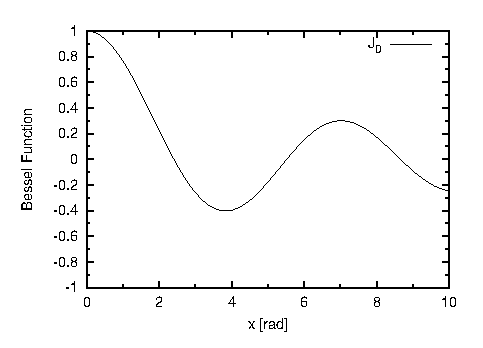
\includegraphics{besj0.eps}}
    \caption{Bessel function, $J_0$.}
    \label{besj0}
  \end{center}
\end{figure}
\clearpage

%
%      FIGURE 2 : J1 Bessel Function
%
\begin{flushright} Fig.~\ref{besj1}~:~ Kawano, T. (Kyushu U.) \end{flushright}
\begin{figure}[b!]
  \begin{center}
    \resizebox{150mm}{!}{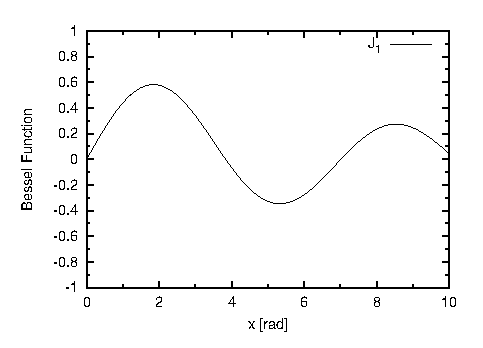
\includegraphics{besj1.eps}}
    \caption{Bessel function, $J_1$.}
    \label{besj1}
  \end{center}
\end{figure}
\clearpage

%
%      FIGURE 3 : Y0 Bessel Function
%
\begin{flushright} Fig.~\ref{besy0}~:~ Kawano, T. (Kyushu U.) \end{flushright}
\begin{figure}[b!]
  \begin{center}
    \resizebox{150mm}{!}{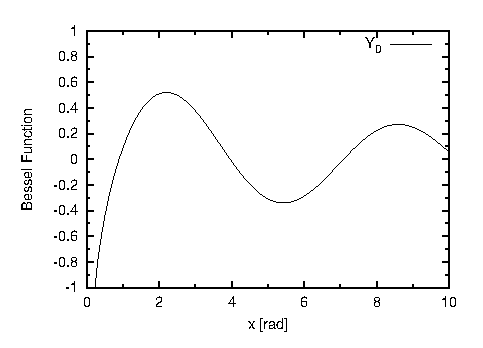
\includegraphics{besy0.eps}}
    \caption{Bessel function, $Y_0$.}
    \label{besy0}
  \end{center}
\end{figure}
\clearpage

%
%      FIGURE 4 : J1 Bessel Function
%
\begin{flushright} Fig.~\ref{besy1}~:~ Kawano, T. (Kyushu U.) \end{flushright}
\begin{figure}[b!]
  \begin{center}
    \resizebox{150mm}{!}{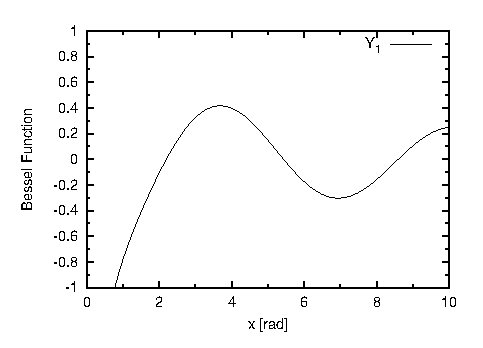
\includegraphics{besy1.eps}}
    \caption{Bessel function, $Y_1$.}
    \label{besy1}
  \end{center}
\end{figure}
\clearpage

%
%      FIGURE 5 : Bessel Functions
%
\begin{flushright} Fig.~\ref{bessel}~:~ Kawano, T. (Kyushu U.) \end{flushright}

\begin{figure}[b!]
  \begin{center}
   \begin{tabular}{cc}
     \resizebox{70mm}{!}{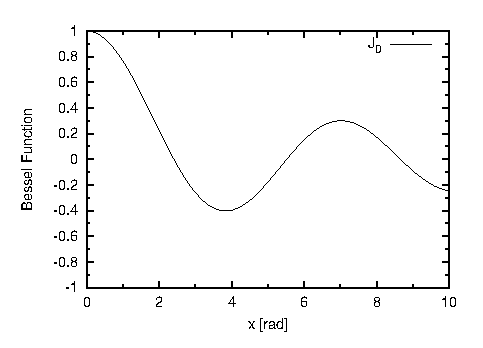
\includegraphics{besj0.eps}} &
     \resizebox{70mm}{!}{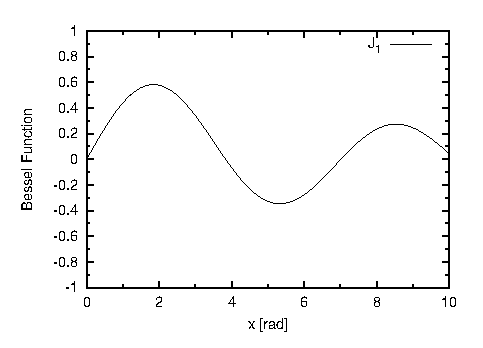
\includegraphics{besj1.eps}} \\
     \resizebox{70mm}{!}{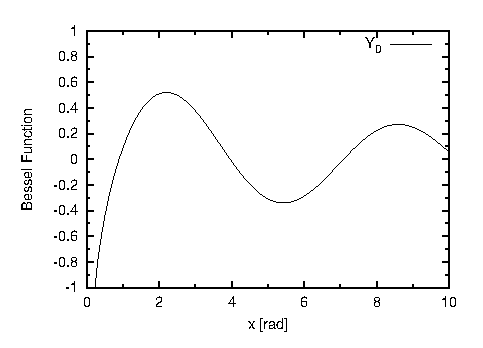
\includegraphics{besy0.eps}} &
     \resizebox{70mm}{!}{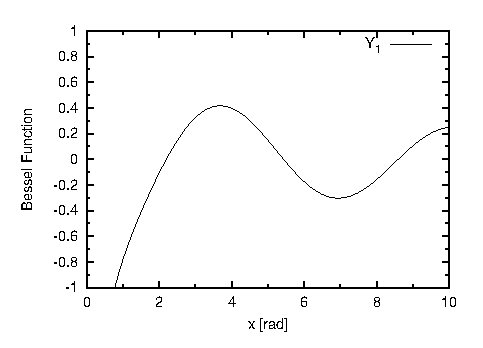
\includegraphics{besy1.eps}} \\
   \end{tabular}
    \caption{Bessel functions, $J_0$, $J_1$, $Y_0$, and $Y_1$.}
    \label{bessel}
  \end{center}
\end{figure}
\clearpage

%
%      FIGURE 6 : Y1 Bessel Function
%
\begin{flushright} Fig.~\ref{besy1a}~:~ Kawano, T. (Kyushu U.) \end{flushright}
\begin{figure}[b!]
  \begin{center}
    \rotatebox{90}{\resizebox{200mm}{!}{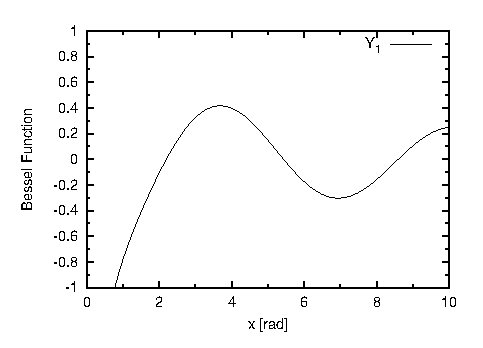
\includegraphics{besy1.eps}}}
    \caption{Bessel function, $Y_1$.}
    \label{besy1a}
  \end{center}
\end{figure}
\clearpage

\end{document}
